\documentclass[nofootinbib,amssymb,amsmath]{revtex4}
\usepackage{mathtools}
\usepackage{amsthm}
\usepackage{algorithm}
\usepackage{algpseudocode}
\usepackage{lmodern}
\usepackage{graphicx}
\usepackage{color}

%Put an averaged random variable between brackets
\newcommand{\ave}[1]{\left\langle #1 \right\rangle}
\newcommand{\HC}{\texttt{HaplotypeCaller}}
\newcommand{\Mutect}{\texttt{Mutect}}
\newcommand{\code}[1]{\texttt{#1}}

\newtheorem{lemma}{Lemma}
\newtheorem{corollary}{Corollary}

\def\SL#1{{\color [rgb]{0,0,0.8} [SL: #1]}}
\def\DB#1{{\color [rgb]{0,0.8,0} [DB: #1]}}

\begin{document}

\title{Local Assembly in HaplotypeCaller and Mutect}
\author{David Benjamin\footnote{The author took no part in development of the methods described below -- credit belongs to several others on the GATK team. }}
\email{davidben@broadinstitute.org}
\affiliation{Broad Institute, 75 Ames Street, Cambridge, MA 02142}

\date{\today}

\begin{abstract}
The GATK tools \HC~and \Mutect~assemble reads aligned within a window of several hundred base pairs into an assembly graph of local variation.  Local haplotypes correspond to paths in this graph, and the downstream likelihood calculations in both tools involve aligning reads to these haplotypes.  Here we describe how this graph is generated.
\end{abstract}

\maketitle

\section{Correcting Reads} \label{correcting-reads}
Read error correction is turned off by default in \HC~ and \Mutect~ and we are not familiar with it, nor have we validated it.  Nonetheless, the code exists and can be turned on.  The idea is as follows: large kmers are good because they contain more phasing information and therefore yield a simpler assembly graph.  For example, two SNVs 20 bases apart with sequenced with error-free reads yield a graph with $2 \times 2 = 4$ paths if $k = 10$ but only $2$ paths if $k = 40$, because the latter spans the phased SNVs.  For example, consider a reference sequence TGAAACGTATTTGGG and an alt sequence with two phased SNVs, TGAAA(C$\rightarrow$T)GTA(T$\rightarrow$C)TTGGG.  If $k=3$ no kmer spans both SNVs and so the assembly graph containing two bubbles, one for each SNV, as in Figure \ref{fig:unphased}.  If $k = 5$, a kmer spans both SNVs and thus only two paths exist in the assembly graph, as in Figure \ref{fig:phased}.

One drawback is that larger kmers are more liable to be lost due to sequencing error simply because they contain more bases\footnote{Another drawback is that longer kmers yield more dangling heads and tails in the graph (see below), especially near the ends of baited regions in exome sequencing.}.  The idea of read error correction is to rescue kmers from the occasional error.

\begin{figure}
\center
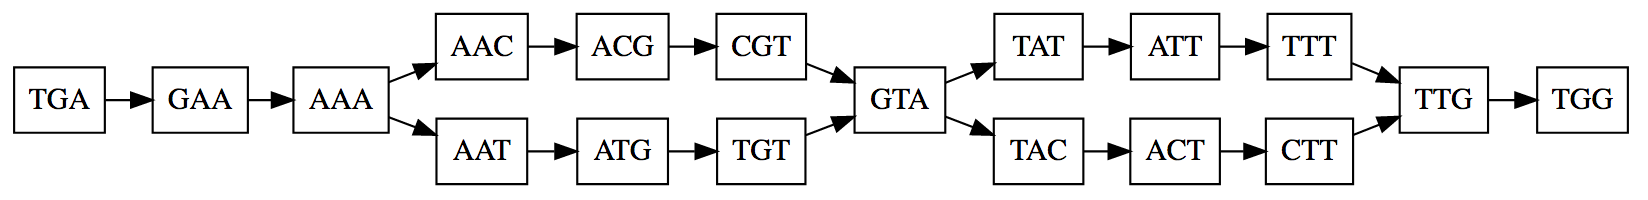
\includegraphics[scale=0.5]{unphased_graph.png}
\caption{Two haplotypes yielding assembly graph with two bubbles and four paths due to too-small $k$.}
\label{fig:unphased}
\end{figure}

\begin{figure}
\center
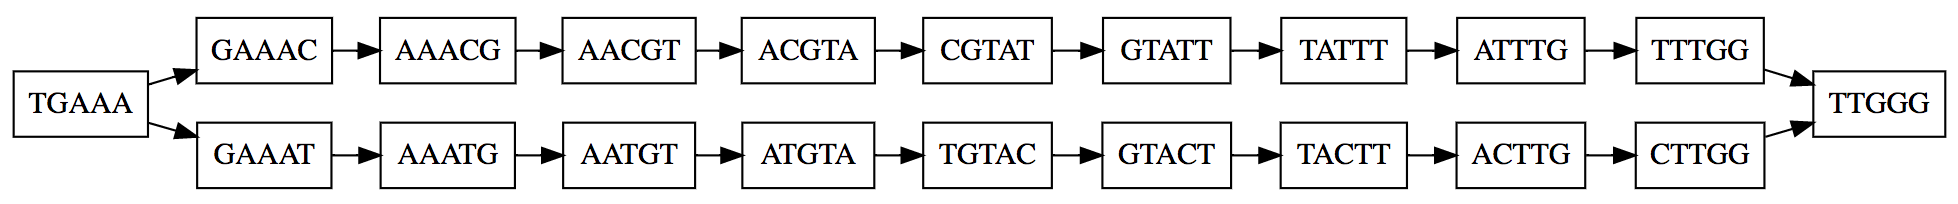
\includegraphics[scale=0.5]{phased_graph.png}
\caption{Two haplotypes yielding assembly graph with a single bubble when $k$ is sufficient to phase variants.}
\label{fig:phased}
\end{figure}

First, the \code{ReadErrorCorrector} kmerizes every read and counts the occurrences of each kmer.  Then it builds a map from kmers to their corrected versions where kmers that appear often\footnote{By default, 20 times or more.  This threshold is set by the \code{minObservationsForKmerToBeSolid} command line argument.} map to themselves and kmers that appear only once\footnote{This is a hardcoded threshold.} map to their nearest neighbor in Hamming distance\footnote{For simplicity we consider only substitution errors, eg the distance between ACGGT and AGGTG is 3} within a maximum of two mismatches\footnote{This is a hardcoded threshold.}.  Kmers that appear between 1 and 20 times are not part of the correction map.

Then, for every base in every read, the \code{ReadErrorCorrector} queries the kmer correction map for each overlapping kmer.  For example, to correct the fourth base of read ACGTATTC if k = 3, it looks at the corrections for CGT, GTA, and TAT at their third, second, and first positions, respectively.  If and only if the corrections are unanimous, the base is corrected.  Note that corrected reads are used only for assembly and the original reads are used downstream.

\section{Building the graph} \label{graph-assembly}
Before we discuss how to construct the graph, let us confess a slight abuse of terminology.  We refer to our assembly graph as a de Bruijn graph, that is, a graph in which the vertices are kmers and two kmers have a directed edge whenever they appear consecutively in a read.  This is almost true (until the last part of assembly when we convert the graph into a more compact sequence graph), but there are a few differences:

\begin{itemize}
\item The edges of our graph record their multiplicity, the number of times the kmers they connect occur consecutively.
\item The kmers of our graph come not just from reads but also the reference haplotype and, in GGA mode (see below), haplotypes generates from the given alleles.
\item A non-unique kmer (see below) may be associated with multiple vertices.
\end{itemize}

Next, the \code{ReadThreadingAssembler} assembles the (corrected) reads over several different kmer sizes specified by the \code{kmerSize} argument\footnote{By default, 10 and 25.  This size is a compromise and no single value is the best choice for all regions.  Large kmers are more likely to be unique and to yield a graph with no cycles, which is especially important in low-complexity regions, but they are more susceptible to decreased sensitivity due to errors and low coverage.}.  If the given kmer sizes fail to produce a graph without cycles, or if more than $1/5$ of the kmers in the graph are not unique in the sequences from which they come\footnote{This uniqueness condition is waived on the last attempt when $k$ has been increased by 60 bases.}, the \code{ReadThreadingAssembler} repeatedly increases $k$ by 10 bases, starting from the largest initial $k$, until assembly succeeds or until $k$ has been increased 6 times, that is, by 60 bases\footnote{These constants, 10 and 6, are hard-coded, but the attempts to increase $k$ can be disabled completely with the \code{dontIncreaseKmerSizesForCycles} argument.}.

The first step is to create a set of sequences to be kmerized and put into the de Bruijn graph.  These sequences are: the reference haplotype, any requested alleles given by the \code{alleles} argument in \HC's ``genotype given alleles" (GGA) mode\footnote{This mode is disabled in \Mutect~ and incompatible with the reference confidence mode of \HC, which is the recommended best practice.  We document it here for completeness.  Before assembly, the GATK engine creates GGA haplotypes by substituting the reference bases with the alt bases from the GGA vcf in the reference haplotype.  These GGA haplotypes are treated as non-reference sequences, that is, as long reads.  The engine does not induce all possible haplotypes obtained from different phasings of GGA alleles, although depending on the kmer size many such haplotypes may appear in the assembly graph.}, and maximal subsequences of reads with base quality at least 10 by default\footnote{This is controlled by the \code{minBaseQualityScore} argument.} and at least one kmer long.  That is, a read with 100 bases and a base of quality 7 at position 70 yields sequences of length 69, 30 if $k = 10$ and a single sequence of length 69 if $k = 40$.  We do not use mate information; that is, a read and its mate yield completely independent sequences, nor do we later post-process the graph using mate information.  This is a potential direction for improvement.

Before building the graph, the \code{ReadThreadingAssembler} finds the set of all kmers that appear more than once in the same sequence i.e. more than once in the reference or in any read.  These are called ``non-unique'' kmers and a kmer that is not non-unique is called ``unique.''  Then each sequence is kmerized starting from the first unique kmer\footnote{Note that a kmer that occurs only once in this particular sequence but more than once in some other sequence in non-unique.}, with the exception that the reference sequence begins at its first kmer, unique or not.  When a new kmer appear a new vertex is added to the graph.  When a unique kmer that is already on the graph appears an edge is added, or the multiplicity of an extant edge is incremented, from the preceding kmer to the current one.  When a non-unique kmer appears and there is already an edge joining the previous kmer to it this edge's multiplicity is incremented, but if an edge does not already exist a completely new vertex and edge are created\footnote{The fact that a non-unique kmer may be associated with multiple vertices on the graph is an important difference between this and a pure de Bruijn graph.}.  The advantage of creating a new vertex for a non-unique kmer rather than re-using an old vertex is that it avoids spurious cycles.  Up to this point, we have strayed from a canonical de Bruijn graph only as noted above.  Note that this is a directed graph of kmers from aligned reads (i.e. aligned to the forward strand of the reference), not a bidirected graph of unaligned reads that could come from either strand, with the complications of associating a kmer with its reverse complement.

\section{Cleaning the Graph} \label{graph-cleaning}
Before deciding on candidate haplotypes, the assembler simplifies the graph with the following heuristics to remove spurious paths and to merge variant paths that diverge from the reference.
\begin{itemize}
\item pruning: The assembler finds all maximal non-branching subgraphs (``chains") and removes those that 1) do not share an edge with the reference path and 2) contain no edges with sufficient multiplicity\footnote{By default 2.  This is controlled by the \code{minPruning} argument.}  While the default multiplicity threshold of 2 is quite permissive, it \textit{does} cause \Mutect~ to lose sensitivity for deletions occurring in a single read\footnote{While a SNV occurring on a single read would not yield a confident somatic variant call, a long deletion in a non-STR context could easily be supported by a single read be due to the tiny probability of its arising from sequencing error.}.

There is a command line flag \code{--adaptive-pruning} to turn on an adaptive pruning algorithm that adjusts itself to both the local depth of coverage and the observed sequencing error rate and removes chains based on a likelihood score.  The score of a chain is the maximum of a left score and a right score, where the score on left (right) end of the chain is the active region determination log likelihood from the \code{Mutect2Engine}, treating the first (last) edge of the chain as a potential variant reads and all other outgoing (incoming) edges of the first (last) vertex in the chain as ref reads.  The adaptive algorithm does this in two passes, where the first pass is used to determine likely errors from which to determine an empirical guess of the error rate.

The adaptive pruning option is extremely useful for samples with high coverage, such as mitochondria and targeted panels, and for samples with variable coverage, such as exomes and RNA.

\item dangling tails: The assembler only outputs haplotypes that start and end with a reference kmer, so it attempts to rescue paths in the graph that do not.  To rescue a ``dangling tails" -- a path that ends in a non-reference kmer vertex -- the assembler first traverses the graph backwards from this vertex to a reference vertex.  If during traversal it encounters a vertex with more than one incoming edge it gives up\footnote{as opposed to doing eg depth-first search of all possible paths back to the reference.}  It also gives up if it encounters a vertex with more than one outgoing edge, that is, if the path branches again after diverging from the reference\footnote{It seems like this could be changed to increase sensitivity.}.  Then it generates the Smith-Waterman alignment of the branching path versus the reference path after the vertex at which they diverge.  If the alignment's CIGAR contains three or fewer elements, that is, if the alignment has at most one indel, the assembly engine attempts to merge the dangling tail back into the reference.

To merge the dangling tail back into the reference path, the assembler finds the beginning of the maximal common suffix of the dangling path and the reference path, that is, the point at which the sequences coverges\footnote{this is \textit{not} where the \textit{paths in the graph} converge (they don't) because kmers in the suffix disagree with the ref at upstream bases.} and adds an edge between the dangling path's vertex and the reference path's vertex at this position.  This means that the graph is no longer a valid de Bruijn graph because the dangling vertex kmer and its succeeding reference vertex kmer do not overlap by $k - 1$ bases.  Nonetheless, this graph yields valid haplotypes when we later ``zip'' the graph's chains (see below) by accumulating the last base of each kmer.

Figure \ref{fig:dangling} shows the result of the tail from alt path ACCTGGA(T$\rightarrow$C)CC being merged back into the reference path.

\begin{figure}
\center
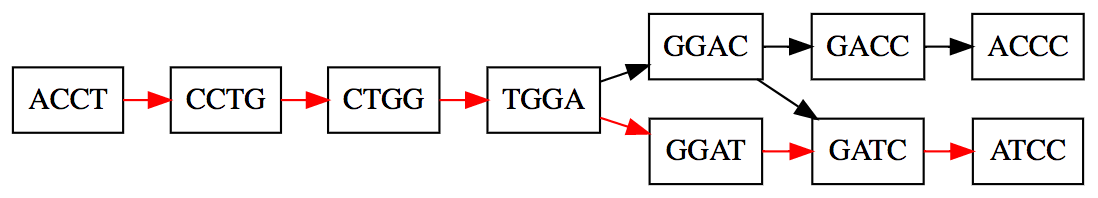
\includegraphics[scale=0.5]{dangling_tail.png}
\caption{A dangling tail merged back into the reference path.  Reference path edges given by red arrows.}
\label{fig:dangling}
\end{figure}

\item dangling heads: This case and its treatment in the assembly engine is the mirror image of dangling tails.

\item non-reference paths: After attempting to merge dangling heads and tails into the reference path, the assembler deletes edges and vertices belonging to dead ends i.e. non-branching subgraphs that start at non-reference source vertices or end at non-reference sink vertices.  This is achieved by performing a breadth-first search of vertices moving forward from the reference source and a breadth-first search of vertices moving backwards from the reference sink and keeping only vertices found in both searches.

\item zipping chains: A de Bruijn graph of kmers is convenient for performing assembly but is inefficient for summarizing the results of assembly.  In this step the assembler converts the de Bruijn graph\footnote{or rather, if dangling paths have been merged, an \textit{almost} de Bruijn graph.} into a sequence graph by combining all vertices in each maximal non-branching subgraph (i.e. each linear chain) into a single vertex containing the sequence implied by those vertices' kmers\footnote{That is, the concatenation of the last bases of all kmers, except for the first vertex which contributes its entire kmer if and only if it is a source.}.  Thus, for example, a de Bruijn graph containing one reference path and one bubble for a single variant, such as the graph of Figure \ref{fig:phased} yields a sequence graph with four vertices: the reference subgraphs before and after the bubble and the two sides of the bubble, as in Figure \ref{fig:zipped}.

\begin{figure}
\center
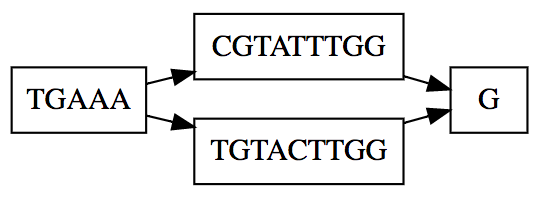
\includegraphics[scale=0.5]{zipped.png}
\caption{A zipped sequence graph.}
\label{fig:zipped}
\end{figure}

\item merging diamonds: The assembler looks for nodes $A$ and $C$ such that multiple paths $A \rightarrow B_i \rightarrow C$ exist and absorbs the common prefix of $\{B_i\}$ into $A$ and the common suffix of $\{ B_i \}$ into $C$.  For example, if $k = 10$ and there was a single SNV bubble in the de Bruijn graph, the zipped sequence graph has a reference source path  ($A$), a reference sink path ($C$) and two sides of the bubble ($B_1$ and $B_2$) that are each $10$ bases long.  Since $B_1$ and $B_2$ differ only in a single base, their common bases can be absorbed into $A$ and $C$ such that $B_1$ and $B_2$ contain only a single base each.  Merging tails works the same way without the terminal vertex $C$ and merging common suffixes works the same way without the terminal vertex $A$.  Figure \ref{fig:diamond} shows the graph of Figure \ref{fig:zipped} after the common suffix GGTT of the two sides of the bubble are absorbed into the terminal vertex.

\begin{figure}
\center
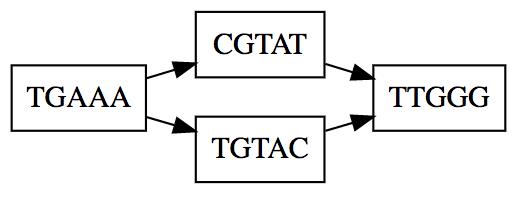
\includegraphics[scale=0.5]{diamond.png}
\caption{A merged diamond.}
\label{fig:diamond}
\end{figure}

\item splitting common prefixes and suffixes: If there are multiple nodes $S_i$ with a common predecessor and successor of the form $S_i = A + x_i + B$, where $A$ is a common prefix, $B$ is a common suffix, and $x_i$ is unique to $S_i$, the assembler splits each $S_i$ such that $A$ and $B$ become independent nodes, with the $x_i$ in between.

\item The clean-up steps of zipping chains, merging diamonds, tails, and common suffixes, and splitting common prefixes and suffixes are repeated until no more transformations occur.

\end{itemize}

When the \code{debugGraphTransformations} argument is used, the assembly engine emits graphviz .dot files for each of the steps above.

\section{Finding Haplotypes} \label{finding-haplotypes}
At this point there is one cleaned sequence graph for each successful kmer size.  For each graph we find the best haplotypes\footnote{This is 128 by default and set by the \code{maxNumHaplotypesInPopulation} argument.} according the following score: the score of a path (haplotype) in a sequence graph is the sum over all branching vertices in the path of the log of the multiplicity of the outgoing edge in the path minus the log of the total multiplicity of all outgoing edges.  This formula is implemented as a recursive depth-first search, sped up via dynamic programming: Starting from the reference source vertex, the haplotype finder adds branching scores and instantiates new haplotype finders for each edge whenever a path diverges and otherwise simply moves to the succeeding vertex without changing the accumulated score.  The recursion ends when a haplotype finder reaches a sink vertex.  The dynamic programming optimization is to cache the best sub-haplotypes found from every previously-reached vertex.  Then, whenever this vertex is reached from a different prefix path, its best suffix paths are queried from the cache.


This description completely defines the best haplotypes; the actual implementation is a somewhat complicated recursive algorithm with lots of polymorphism.

\end{document}